\documentclass{article}
\usepackage[margin=1in]{geometry}
\usepackage{amsmath}
\usepackage{amssymb}
\usepackage{graphicx}
\usepackage{svg}
\usepackage{comment}
\usepackage{float}
\usepackage{cancel}
\usepackage{enumerate}
\usepackage[italicdiff]{physics}
\usepackage{dsfont}
\usepackage{hyperref}
\usepackage{siunitx}
% Display code
\usepackage{minted}
\usepackage{listings}
% Display graphs/figures
\usepackage{tikz}
\usepackage{hhline}
\hypersetup{
    colorlinks=true,
    linkcolor=blue,
    filecolor=blue,
    urlcolor=blue,
}
% Display boxes
\usepackage{tcolorbox}
\definecolor{lblue}{rgb}{0, 0.69, 1}

% Static title
\newtcolorbox{quickcheck}{fonttitle=\bfseries, title=Quick check}
\newtcolorbox{note}{colback=blue!5!white, colframe=blue!75!black,
fonttitle=\bfseries, title=Note}
\newtcolorbox{keyideas}{colback=green!5!white, colframe=green!75!black,
fonttitle=\bfseries, title=Key ideas}
\newtcolorbox{summary}{colback=green!5!white, colframe=green!75!black,
fonttitle=\bfseries, title=Summary}
\newtcolorbox{admin}{colback=yellow!5!white, colframe=yellow!90!black,
fonttitle=\bfseries, title=Administrivia}
% Editable title
\newtcolorbox{theorem}[1]{colback=lblue!5!white, colframe=lblue!75!black,
fonttitle=\bfseries, title=#1}
\newtcolorbox{problem}[1]{colback=red!5!white, colframe=red!75!black,
fonttitle=\bfseries, title=#1}
\newtcolorbox{example}[1]{colback=white, colframe=black,
fonttitle=\bfseries, title=#1}
\newtcolorbox{exercise}[1]{colback=orange!5!white, colframe=orange!95!black,
fonttitle=\bfseries, title=#1}
\newtcolorbox{strategy}[1]{colback=yellow!5!white, colframe=yellow!50!white, coltitle=black,
fonttitle=\bfseries, title=#1}
\newtcolorbox{definition}[1]{colback=green!5!white, colframe=green!75!black,
fonttitle=\bfseries, title=#1}

\newcommand{\sign}{\mathrm{sign}}

\newcommand{\RR}{\mathbb{R}}
\newcommand{\CC}{\mathbb{C}}

\newcommand{\cF}{\mathcal{F}}

% Start doc

\begin{document}
\title{Phyll-in Notes, Lecture 4: Graphs, DFS, SCCs}
\author{CS124 - Spring 2023}
\date{Andrew Holmes --- 10 January 2023 --- version 1.0}
\maketitle

\tableofcontents

% \section{Admininstriva/Key ideas}
% \begin{admin}
%     \begin{itemize}
%         \item PSET 1 due today
%         \item PSET 2 out later today (due in 2 weeks)
%     \end{itemize}
% \end{admin}

% \begin{keyideas}
%     \begin{itemize}
%         \item What is a graph? Why might graphs be useful? How can we represent graphs?
%         \item Depth-First Search (DFS)
%         \begin{itemize}
%             \item Correctness, time \& space complexity
%             \item Properties \& types of edges
%             \item Topological sort
%         \end{itemize}
%         \item Strongly connected components (SCCs)
%     \end{itemize}
% \end{keyideas}

\newpage
\section{Graphs}
\subsection{Graph introduction}
A graph is a data structure consisting of a set of vertices and a set of edges between vertices. 
\begin{figure}[h]
    \centering
    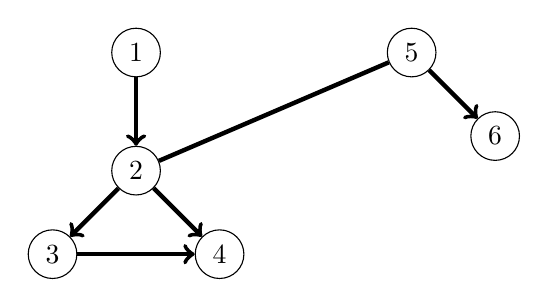
\begin{tikzpicture}[main/.style = {draw, circle}, node distance={15mm}] 
        \node[main] (1) {$1$}; 
        \node[main] (2) [below of=1] {$2$};
        \node[main] (3) [below left of=2] {$3$};
        \node[main] (4) [below right of=2] {$4$};
        \node[main] (5) [xshift=3.5cm] {$5$};
        \node[main] (6) [below right of=5] {$6$};
        \draw[->, ultra thick] (1) -- (2);
        \draw[->, ultra thick] (2) -- (3);
        \draw[->, ultra thick] (2) -- (4);
        \draw[->, ultra thick] (3) -- (4);
        \draw[->, ultra thick] (5) -- (6);
        \draw[-, ultra thick] (5) -- (2);
    \end{tikzpicture}
    \caption{A basic graph}
    \label{graph-intro-graph}
\end{figure}

\vspace{8cm}

\begin{quickcheck}
    Let's consider the graph in \ref{graph-intro-graph}. Fill in $V(G)$ and $E(G)$ for this graph:
    \begin{align*}
        V(G) &= \{ \qquad \qquad \qquad \qquad \}\\
        E(G) &= \{\qquad \qquad \qquad \qquad \qquad \qquad \qquad \qquad \}
    \end{align*}
\end{quickcheck}

\begin{problem}{Problem 1: Modelling problems with graphs}
    What are some things we might model with graphs?
\end{problem}


\newpage

\subsection{Graph representation}
\begin{problem}{Problems 2 \& 3: Graph representation}
    How can we represent a graph? How should we represent a graph?
\end{problem}

\vspace{9cm}

\begin{example}{Graph representation example}
    \begin{center}
    \begin{minipage}{.25\linewidth}

    \centering
    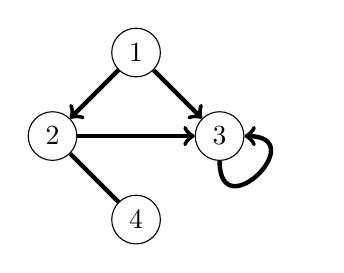
\begin{tikzpicture}[main/.style = {draw, circle}, node distance={15mm}] 
        \node[main] (1) {$1$};
        \node[main] (2) [below left of=1] {$2$};
        \node[main] (3) [below right of=1] {$3$};
        \node[main] (4) [below right of=2] {$4$};
        \draw[->, ultra thick] (1) -- (2);
        \draw[->, ultra thick] (2) -- (3);
        \draw[->, ultra thick] (1) -- (3);
        \draw[->, ultra thick] (3) to [out=270,in=0,looseness=5] (3);
        \draw[-, ultra thick] (2) to (4);
    \end{tikzpicture}
    \caption{Example graph}
    \label{graph-rep-ex}
\end{minipage}%
\begin{minipage}{.3\linewidth}
    \centering
    \begin{tabular}{|c||c|c|c|c|}
         \hline
         Vertex & 1 & 2 & 3 & 4 \\
         \hhline{|=||=|=|=|=|}
         1 & 0 & 1 & 1 & 0\\
         2 & 0 & 0 & 1 & 1\\
         3 & 0 & 0 & 1 & 0\\
         4 & 0 & 1 & 0 & 0\\
         \hline
    \end{tabular}
    \vspace{2mm}
    
    \caption{Adjacency matrix corresponding to graph}
    \label{tab:my_label}
\end{minipage}
\begin{minipage}{.25\linewidth}
    \centering
    \includegraphics[scale=0.35]{adj-list-ex.PNG}
    
    \caption{Adjacency list corresponding to graph}
    \label{tab:my_label}
\end{minipage}
\end{center}
\end{example}


\begin{note}
    We will often classify graphs into certain types:
    \begin{itemize}
        \setlength\itemsep{0.05em} 
        \item \textbf{Directed or undirected} (see 1.1: Graph introduction)
        \item \textbf{Cyclic or acyclic} - does the graph contain one or more cycles?
        \item \textbf{Connected} - exists a \textbf{path} between every pair of vertices (not necessarily a direct edge)
        \item \textbf{Complete} - exists an \textbf{edge} between every pair of vertices
        \item \textbf{Tree} - an undirected graph where any two vertices are connected by \textbf{exactly} one path
        \item \textbf{DAG} - a Directed Acyclic Graph.
    \end{itemize}
\end{note}

\newpage
\section{Depth-First Search (DFS)}

\subsection{DFS introduction}

There are two fundamental algorithms for searching a graph: \textbf{depth-first search} and \textbf{breadth-first search}. We will explore depth-first search this lecture, and breadth-first search next lecture.

Depth-First Search follows edges from vertex to vertex until it reaches a vertex it has already visited or a vertex with no outgoing edges, at which point it backtracks (reverses its steps) until it reaches a vertex that has outgoing edges that it has not explored yet. One famous example of DFS is exploring mazes:

\noindent
\begin{minipage}{.33\linewidth}
    \includegraphics[scale=0.37]{maze-DFS-1.PNG}
    
    % \caption{}
    \label{tab:my_label}
\end{minipage}
\begin{minipage}{.33\linewidth}
    \includegraphics[scale=0.37]{maze-DFS-2.PNG}
    
    % \caption{}
    \label{tab:my_label}
\end{minipage}
\begin{minipage}{.33\linewidth}
    \includegraphics[scale=0.37]{maze-DFS-3.PNG}
    
    % \caption{}
    \label{tab:my_label}
\end{minipage}

Looking at this example, DFS on this maze chooses to go right initially, and it explores this path as far as it can go, then backtracks back to the start square. Here there is another available path, so it explores down this path in the second image. At the next junction, it chooses to go right, and again explores this path until it can go no further before backtracking, and the same again in the third image. 

\begin{note}
    We can represent this maze as a graph, hence allowing us to run DFS! For example, the top left corner can be represented as the following graph:
    
    \centering
    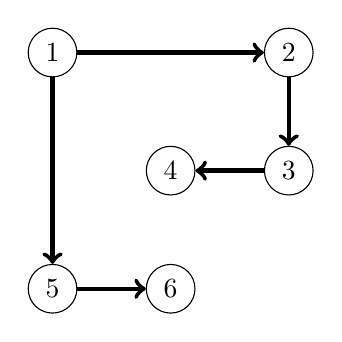
\begin{tikzpicture}[main/.style = {draw, circle}, node distance={15mm}] 
        \node[main] (1) {$1$};
        \node[main] (2) [right of=1, xshift=1.5cm] {$2$};
        \node[main] (3) [below of=2] {$3$};
        \node[main] (4) [left of=3] {$4$};
        \node[main] (5) [below of=1, yshift=-1.5cm] {$5$};
        \node[main] (6) [right of=5] {$6$};
        \draw[->, ultra thick] (1) -- (2);
        \draw[->, ultra thick] (2) -- (3);
        \draw[->, ultra thick] (3) -- (4);
        \draw[->, ultra thick] (1) to (5);
        \draw[->, ultra thick] (5) to (6);
    \end{tikzpicture}

    Our DFS started at vertex $1$, then went $1 \to 2 \to 3 \to 4$. $4$ is a leaf vertex/has no outgoing edges, so it backtracked to $1$. $1$ has another edge it can follow, so it searched that branch, following $1 \to 5 \to 6$ and so on.
\end{note}

\subsection{DFS and stacks}

Depth-First Search uses a \textbf{stack} to keep track of which vertices to explore next. A stack is a \textbf{last in, first out (LIFO)} data structure. This means that the last item we add to the stack is always the first to be removed. We generally refer to adding to a stack as \textbf{pushing/appending} to a stack, and removing an element as \textbf{popping} an element.

For example, in the dining hall the staff create a stack of trays. The last clean tray added is at the top, and when you arrive in the dining hall, the tray you collect is the top one (the last added). The person afer you collects a tray that was added to the stack before your one. If the stack was getting low, staff might come and add several more trays, such that the tray at the very bottom might have been added first, but never gets used. In this example, it would be possible, albeit a massive pain trying to remove the first clean tray from the bottom without removing the others. People here could break the normal stack order - when programming a stack, it's common to use an abstraction barrier to prevent actions like these. 

In DFS, when we find a vertex and explore its edges, we add each unvisited vertex accessible from one of these edges to the stack. We then pop (remove) one of them from the stack (the last one added), and repeat the process until our stack is empty. Let's explore an example in detail.

\begin{example}{DFS example}
    Let's break down how DFS ran on the maze graph:

    \centering

    \begin{minipage}{0.4\linewidth}
        \centering
        \textbf{Diagram}
    \end{minipage}
    \begin{minipage}{0.4\linewidth}
    \centering
        \textbf{Explanation}
    \end{minipage}
    \begin{minipage}{0.15\linewidth}
    \centering
        \textbf{Stack at end of step}
    \end{minipage} \\
    
    \begin{minipage}{0.4\linewidth}
    \centering
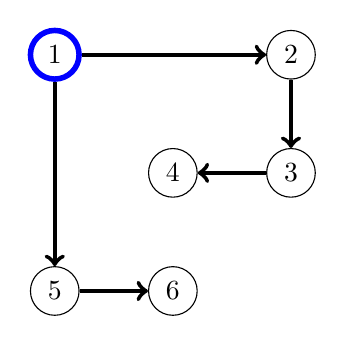
\begin{tikzpicture}[main/.style = {draw, circle}, node distance={15mm},   blacknode/.style={shape=circle, draw=black, line width=2},                              bluenode/.style={shape=circle, draw=blue, line width=2}]        \centering
        \node[bluenode] (1) {$1$};
        \node[main] (2) [right of=1, xshift=1.5cm] {$2$};
        \node[main] (3) [below of=2] {$3$};
        \node[main] (4) [left of=3] {$4$};
        \node[main] (5) [below of=1, yshift=-1.5cm] {$5$};
        \node[main] (6) [right of=5] {$6$};
        \draw[->, ultra thick] (1) -- (2);
        \draw[->, ultra thick] (2) -- (3);
        \draw[->, ultra thick] (3) -- (4);
        \draw[->, ultra thick] (1) to (5);
        \draw[->, ultra thick] (5) to (6);
    \end{tikzpicture}
    \end{minipage}
    \begin{minipage}{0.4\linewidth}
    \centering
        We start with the source vertex, and set it as visited. We push the two vertices we can reach from $1$ to the stack in some order, in this case $5$ and then $2$. 
    \end{minipage}
    \begin{minipage}{0.15\linewidth}
    \centering
        $\{5, 2\}$
    \end{minipage}   \\
    \begin{minipage}{0.4\linewidth}
    \centering
    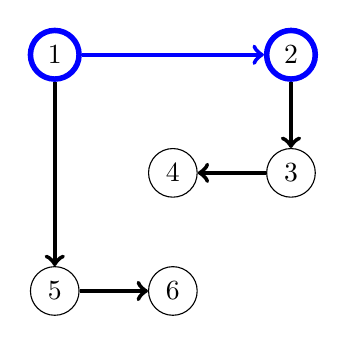
\begin{tikzpicture}[main/.style = {draw, circle}, node distance={15mm},                               bluenode/.style={shape=circle, draw=blue, line width=2}] 
    \centering
        \node[bluenode] (1) {$1$};
        \node[bluenode] (2) [right of=1, xshift=1.5cm] {$2$};
        \node[main] (3) [below of=2] {$3$};
        \node[main] (4) [left of=3] {$4$};
        \node[main] (5) [below of=1, yshift=-1.5cm] {$5$};
        \node[main] (6) [right of=5] {$6$};
        \draw[->, ultra thick, blue] (1) -- (2);
        \draw[->, ultra thick] (2) -- (3);
        \draw[->, ultra thick] (3) -- (4);
        \draw[->, ultra thick] (1) to (5);
        \draw[->, ultra thick] (5) to (6);
    \end{tikzpicture}
    \end{minipage}
    \begin{minipage}{0.4\linewidth}
    \centering
        We now pop $2$ from the stack and set it as visited. We push $3$ to the stack since it is the only unvisited vertex we can reach from $2$.
    \end{minipage}
    \begin{minipage}{0.15\linewidth}
    \centering
        $\{5, 3\}$
    \end{minipage}    \\
    \begin{minipage}{0.4\linewidth}
    \centering
    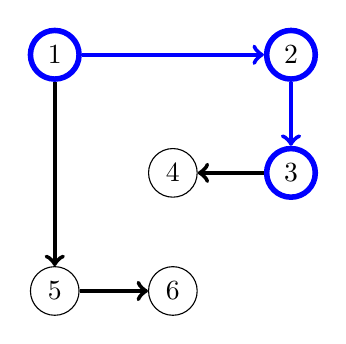
\begin{tikzpicture}[main/.style = {draw, circle}, node distance={15mm},                               bluenode/.style={shape=circle, draw=blue, line width=2}] 
    \centering
        \node[bluenode] (1) {$1$};
        \node[bluenode] (2) [right of=1, xshift=1.5cm] {$2$};
        \node[bluenode] (3) [below of=2] {$3$};
        \node[main] (4) [left of=3] {$4$};
        \node[main] (5) [below of=1, yshift=-1.5cm] {$5$};
        \node[main] (6) [right of=5] {$6$};
        \draw[->, ultra thick, blue] (1) -- (2);
        \draw[->, ultra thick, blue] (2) -- (3);
        \draw[->, ultra thick] (3) -- (4);
        \draw[->, ultra thick] (1) to (5);
        \draw[->, ultra thick] (5) to (6);
    \end{tikzpicture}
    \end{minipage}
        \begin{minipage}{0.4\linewidth}
    \centering
        We now pop $3$ from the stack and set it as visited.  We push $4$ to the stack since it is the only unvisited vertex we can reach from $3$.
    \end{minipage}
    \begin{minipage}{0.15\linewidth}
    \centering
        $\{5, 4\}$
    \end{minipage}\\
    \begin{minipage}{0.4\linewidth}
    \centering
    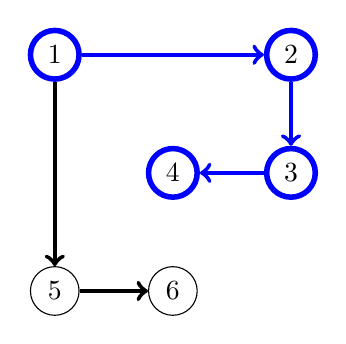
\begin{tikzpicture}[main/.style = {draw, circle}, node distance={15mm},                               bluenode/.style={shape=circle, draw=blue, line width=2}] 
    \centering
        \node[bluenode] (1) {$1$};
        \node[bluenode] (2) [right of=1, xshift=1.5cm] {$2$};
        \node[bluenode] (3) [below of=2] {$3$};
        \node[bluenode] (4) [left of=3] {$4$};
        \node[main] (5) [below of=1, yshift=-1.5cm] {$5$};
        \node[main] (6) [right of=5] {$6$};
        \draw[->, ultra thick, blue] (1) -- (2);
        \draw[->, ultra thick, blue] (2) -- (3);
        \draw[->, ultra thick, blue] (3) -- (4);
        \draw[->, ultra thick] (1) to (5);
        \draw[->, ultra thick] (5) to (6);
    \end{tikzpicture}
    \end{minipage}
    \begin{minipage}{0.4\linewidth}
    \centering
        We now pop $4$ from the stack and set it as visited.  There is nowhere to go from $4$, so we push nothing to the stack. Since only $5$ remains on the stack, we will explore $5$ next - this is where we encounter the idea of backtracking: we just explored $4$, but now we go back to one of the outgoing edges from $1$ since we have run out of paths on this branch.
    \end{minipage}
    \begin{minipage}{0.15\linewidth}
    \centering
        $\{5\}$
    \end{minipage}\\
    \begin{minipage}{0.4\linewidth}
    \centering
    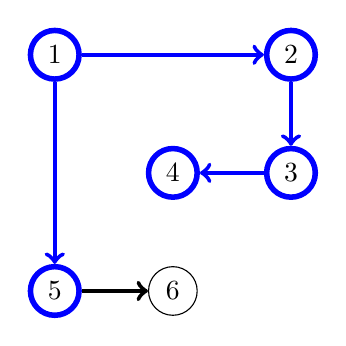
\begin{tikzpicture}[main/.style = {draw, circle}, node distance={15mm},                               bluenode/.style={shape=circle, draw=blue, line width=2}] 
    \centering
        \node[bluenode] (1) {$1$};
        \node[bluenode] (2) [right of=1, xshift=1.5cm] {$2$};
        \node[bluenode] (3) [below of=2] {$3$};
        \node[bluenode] (4) [left of=3] {$4$};
        \node[bluenode] (5) [below of=1, yshift=-1.5cm] {$5$};
        \node[main] (6) [right of=5] {$6$};
        \draw[->, ultra thick, blue] (1) -- (2);
        \draw[->, ultra thick, blue] (2) -- (3);
        \draw[->, ultra thick, blue] (3) -- (4);
        \draw[->, ultra thick, blue] (1) to (5);
        \draw[->, ultra thick] (5) to (6);
    \end{tikzpicture}    
    \end{minipage}
    \begin{minipage}{0.4\linewidth}
    \centering
        We now pop $5$ from the stack and set it as visited.  We push $6$ to the stack since it is the only unvisited vertex we can reach from $5$.
    \end{minipage}
    \begin{minipage}{0.15\linewidth}
    \centering
        $\{6\}$
    \end{minipage}\\
\end{example}

\newpage

\subsection{DFS pseudocode}

\begin{strategy}{DFS pseudocode (attempt 1)}
    Here's an attempt at writing some pseudocode for DFS:
    \begin{lstlisting}
    def search(v):
	explored(v) = 1
	previsit(v)
	for (v,w) in E:
		if explored(w) == 0:
			search(w)
	postvisit(v)
\end{lstlisting}
\end{strategy}
\begin{problem}{Problem 4: DFS pseudocode}
    Is this guaranteed to reach every node in a graph? When will it search all of $G$?
\end{problem}


\newpage
\begin{strategy}{DFS pseudocode fix}
    Let's fix our pseudocode for DFS. We will use the previous version as a helper function to the main DFS function to fix our problems:
    \begin{lstlisting}[mathescape=true]
def search(v):
    explored(v) = 1
    previsit(v)
    for (v,w) in E:
        if explored(w) == 0:
            search(w)
    postvisit(v)
    \end{lstlisting}  

    \textcolor{red}{Complete the pseudocode for DFS to fix the problems from our first attempt!}
    \begin{lstlisting}
def DFS(G):
    for v in V(G):
        explored(v) = 0
    \end{lstlisting}
    \vspace{-3mm}
    \begin{tcolorbox}
    \vspace{2cm}
    \end{tcolorbox}
\end{strategy}

\begin{note}
    Looking at our pseudocode above, there is no clear implementation or usage of a stack. This is because, by using recursion, we are using the \textbf{calling stack} implicitly to handle our stack for us. \lstinline{search(v)} is on the calling stack before \lstinline{search(w)}, and this is where the stack is hidden in this implementation. Here's an iterative implementation with an explicit stack, although without previsit/postvisit as this is trickier to do iteratively.

    \begin{lstlisting}
def DFS(self,s):
    for v in V(G):
        explored(v) = 0
    stack = []
    stack.append(s)
    while (stack not empty):
        v = stack.pop()
        explored(v) = 1
        for (v, w) in E(G):
            if (explored(w) == 0:
                stack.append(w)
    \end{lstlisting}
    
\end{note}

\subsection{DFS time complexity}

\begin{problem}{Problem 5: DFS time complexity}
    How long does DFS take to run?
\end{problem}


\newpage
\subsection{Postvisit/previsit}
\vspace{3.5cm}

\begin{example}{Previsit/postvisit example}
    Let's run DFS on the following graph, assuming it picks $1$ as the initial vertex and it will break ties in ascending vertex order (lowest vertex will always be picked first).

    \vspace{2mm}
    \begin{minipage}{0.5\linewidth}
    \centering
    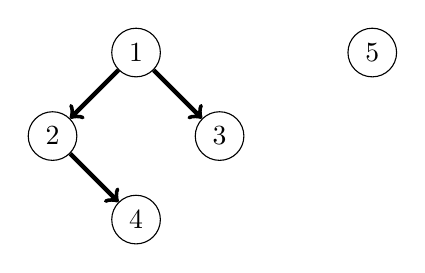
\begin{tikzpicture}[main/.style = {draw, circle}, node distance={15mm}] 
        \node[main] (1) {$1$};
        \node[main] (2) [below left of=1] {$2$};
        \node[main] (3) [below right of=1] {$3$};
        \node[main] (4) [below right of=2] {$4$};
        \node[main] (5) [xshift=3cm] {$5$};
        \draw[->, ultra thick] (1) -- (2);
        \draw[->, ultra thick] (1) -- (3);
        \draw[->, ultra thick] (2) -- (4);
    \end{tikzpicture}
    \end{minipage}
    \begin{minipage}{0.5\linewidth}
    \centering
    \begin{tabular}{|c|c|c|}
        \hline
        Vertex & Previsit & Postvisit  \\
        \hline
        1 &  &  \\
        2 &  &  \\
        3 &  &  \\
        4 &  &  \\
        5 &  &   \\
        \hline
    \end{tabular}
    \end{minipage}
\end{example}


\subsection{Types of edges}

When we run DFS on a graph, we can categorize the edges of the graph into 4 categories:

\begin{itemize}
    \item \textbf{Tree (actually forest) edges}: 
    \item \textbf{Forward edges}: 
    \item \textbf{Back edges}: 
    \item \textbf{Cross edges}: 
\end{itemize}

\begin{exercise}{\text{Exercise: Label tree, forward, back and cross edges}}
    \centering
        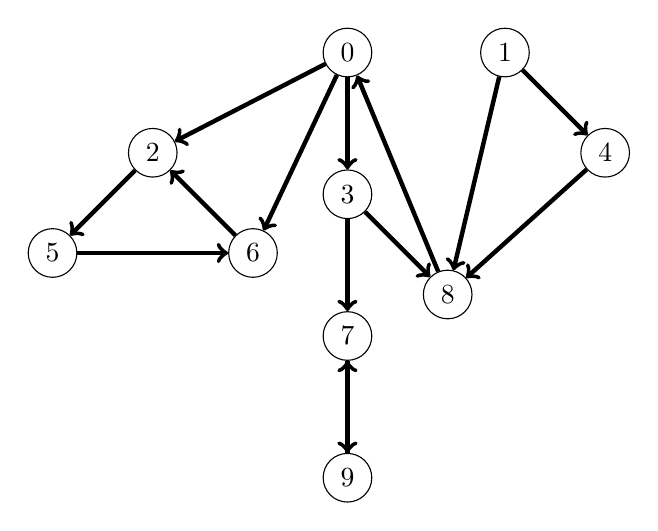
\begin{tikzpicture}[main/.style = {draw, circle}, node distance={18mm},   blacknode/.style={shape=circle, draw=black, line width=2},
  bluenode/.style={shape=circle, draw=blue, line width=2},
  yellownode/.style={shape=circle, draw=yellow, line width=2},
  rednode/.style={shape=circle, draw=red, line width=2}] 
        \node[main] (0) {$0$};
        \node[main] (1) [xshift=2cm] {$1$};
        \node[main] (2) [below left of=0, xshift=-1.2cm] {$2$};
        \node[main] (3) [below of=0] {$3$};
        \node[main] (4) [below right of=1] {$4$};
        \node[main] (5) [below left of=2] {$5$};
        \node[main] (6) [below right of=2] {$6$};
        \node[main] (7) [below of=3] {$7$};
        \node[main] (8) [below right of=3] {$8$};
        \node[main] (9) [below of=7] {$9$};
        \draw[->, ultra thick] (0) -- (2);
        \draw[->, ultra thick] (2) -- (5);
        \draw[->, ultra thick] (5) -- (6);
        \draw[->, ultra thick] (6) -- (2);
        \draw[->, ultra thick] (0) -- (3);
        \draw[->, ultra thick] (0) -- (6);
        \draw[->, ultra thick] (3) -- (7);
        \draw[->, ultra thick] (7) -- (9);
        \draw[->, ultra thick] (3) -- (8);
        \draw[->, ultra thick] (8) -- (0);
        \draw[->, ultra thick] (1) -- (4);
        \draw[->, ultra thick] (4) -- (8);
        \draw[->, ultra thick] (1) -- (8);
        \draw[->, ultra thick] (9) -- (7);
    \end{tikzpicture}
    \label{fig:my_label}
\end{exercise}

\newpage

\subsection{DFS properties}
DFS has a number of useful properties that we will use in the future:

\begin{theorem}{DFS property 1}
    \vspace{8mm}
\end{theorem}

\textbf{Proof}:

\vspace{4cm}

\begin{theorem}{DFS property 2}
      \vspace{8mm}
\end{theorem}

\textbf{Proof}:

\vspace{4cm}


\begin{problem}{Problem 6: DFS \& back edges}
    Is it possible that one DFS of a graph G yields a back edge, but another DFS yields no back edges?
\end{problem}



\newpage
\subsection{Topological sort}

\begin{problem}{Problen 7: Topological sort}
    Let's suppose you have a list of tasks where some tasks must be done before others. Is it always possible to order them?
\end{problem}

\vspace{2cm}


\begin{problem}{Problem 8: Topogical sort 2}
    Topological Sort: you have a list of tasks; some tasks must be done before others. How to order them?
\end{problem}

\vspace{2cm} 

\begin{definition}{Definition: Topological sort/ordering}
    \vspace{8mm}
\end{definition}


\begin{strategy}{Topological sort algorithm}
    \begin{enumerate}
        \item 
        \item 
    \end{enumerate}   
\end{strategy}

\textbf{Proof that this gives a topological sort}:

\vspace{22mm}

\begin{example}{Topological sort example} 
    \centering
    \begin{minipage}{0.4\linewidth}
    \centering
    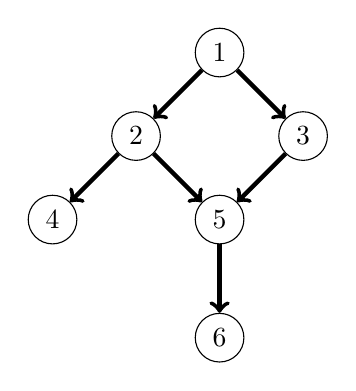
\begin{tikzpicture}[main/.style = {draw, circle}, node distance={15mm}] 
        \node[main] (1) {$1$};
        \node[main] (2) [below left of=1] {$2$};
        \node[main] (3) [below right of=1] {$3$};
        \node[main] (4) [below left of=2] {$4$};
        \node[main] (5) [below right of=2] {$5$};
        \node[main] (6) [below of=5] {$6$};
        \draw[->, ultra thick] (1) -- (2);
        \draw[->, ultra thick] (1) -- (3);
        \draw[->, ultra thick] (2) -- (4);
        \draw[->, ultra thick] (2) -- (5);
        \draw[->, ultra thick] (3) -- (5);
        \draw[->, ultra thick] (5) -- (6);
    \end{tikzpicture}
    \end{minipage}
    \begin{minipage}{0.4\linewidth}
    \centering
    One possible topological ordering for this graph is: $[1, 2, 3, 4, 5, 6]$. However, there are many more! For example, $[1, 3, 2, 5, 6, 4]$.
    \end{minipage}
\end{example}


\newpage

\section{Strongly Connected Components (SCCs)}
\subsection{Strongly Connected Components introduction}

\begin{definition}{Definition: Strongly Connected Component}
   \vspace{8mm}
\end{definition}

\begin{problem}{Problem 9: Identify SCCs}
    What are the SCCs of the following graph?

    \vspace{5mm}
    
    \centering
        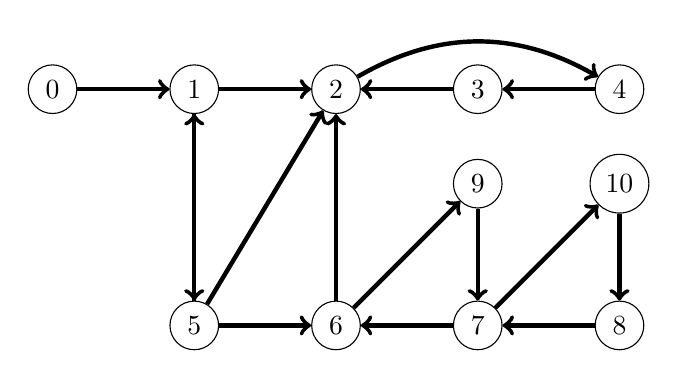
\begin{tikzpicture}[main/.style = {draw, circle}, node distance={18mm},   blacknode/.style={shape=circle, draw=black, line width=2},
                              bluenode/.style={shape=circle, draw=blue, line width=2},
                              greennode/.style={shape=circle, draw=green, line width=2},
                              rednode/.style={shape=circle, draw=red, line width=2}] 
        \node[main] (0) {$0$};
        \node[main] (1) [right of=0] {$1$};
        \node[main] (2) [right of=1] {$2$};
        \node[main] (3) [right of=2] {$3$};
        \node[main] (4) [right of=3] {$4$};
        \node[main] (5) [below of=1, yshift=-1.2cm] {$5$};
        \node[main] (6) [right of=5] {$6$};
        \node[main] (7) [right of=6] {$7$};
        \node[main] (8) [right of=7] {$8$};
        \node[main] (9) [above of=7] {$9$};
        \node[main] (10) [above of=8] {$10$};
        \draw[->, ultra thick] (0) -- (1);
        \draw[->, ultra thick] (1) -- (2);
        \draw[->, ultra thick] (3) -- (2);
        \draw[->, ultra thick] (4) -- (3);
        \draw[->, ultra thick] (2) to [out=30, in=150] (4);
        \draw[->, ultra thick] (1) -- (5);
        \draw[->, ultra thick] (5) -- (1);
        \draw[->, ultra thick] (5) -- (2);
        \draw[->, ultra thick] (5) -- (6);
        \draw[->, ultra thick] (6) -- (2);
        \draw[->, ultra thick] (6) -- (9);
        \draw[->, ultra thick] (7) -- (6);
        \draw[->, ultra thick] (7) -- (10);
        \draw[->, ultra thick] (10) -- (8);
        \draw[->, ultra thick] (9) -- (7);
        \draw[->, ultra thick] (8) -- (7);
    \end{tikzpicture}

    \vspace{12mm}
\end{problem}

\begin{problem}{Problem 10: SCC graph as a DAG}
    Suppose you make a new graph $G’$ whose vertices are the SCCs of $G$. Prove that $G’$ is a DAG.
\end{problem}

\textbf{Proof}:

\vspace{3cm}

\newpage
\subsection{Finding SCCs}

To help us with an algorithm to find SCCs, we will quickly prove two theorems:

\begin{theorem}{SCC Theorems}
\begin{enumerate}
    \item If you start DFS from a vertex in a sink SCC, you visit exactly that SCC.
    \item The vertex with the highest postorder number is in a source SCC.
\end{enumerate}
\end{theorem}

\textbf{Proof of 1}: 
\vspace{2cm}

\textbf{Proof of 2}: 

\vspace{3cm}

Now we combine these two into an algorithm to find SCCs:

\begin{strategy}{SCC-finding algorithm}
\begin{enumerate}
    \item 
    \item
\end{enumerate}
\vspace{3mm}
\end{strategy}
    
\vspace{3cm}

\begin{quickcheck}
    \centering
    \begin{minipage}{.35\linewidth}
    \centering
    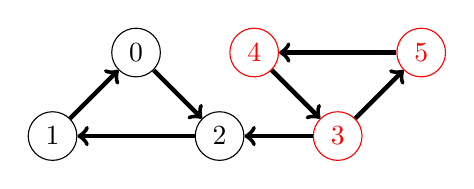
\begin{tikzpicture}[main/.style = {draw, circle}, node distance={15mm},   blacknode/.style={shape=circle, draw=black, line width=2},
                              bluenode/.style={shape=circle, draw=blue, line width=2},
                              greennode/.style={shape=circle, draw=green, line width=2},
                              rednode/.style={shape=circle, draw=red, line width=2}] 
        \node[main] (0) {$0$};
        \node[main] (1) [below left of=0] {$1$};
        \node[main] (2) [below right of=0] {$2$};
        \node[main, red] (3) [right of=2] {$3$};
        \node[main, red] (4) [above left of=3] {$4$};
        \node[main, red] (5) [above right of=3] {$5$};
        \draw[->, ultra thick] (1) -- (0);
        \draw[->, ultra thick] (2) -- (1);
        \draw[->, ultra thick] (0) -- (2);
        \draw[->, ultra thick] (3) -- (2);
        \draw[->, ultra thick] (4) -- (3);
        \draw[->, ultra thick] (5) -- (4);
        \draw[->, ultra thick] (3) -- (5);
    \end{tikzpicture}
    \caption{$G^R$}

    \end{minipage}
    \begin{minipage}{.35\linewidth}
    \centering
    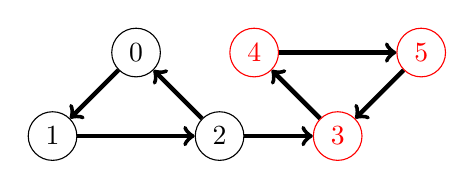
\begin{tikzpicture}[main/.style = {draw, circle}, node distance={15mm},   blacknode/.style={shape=circle, draw=black, line width=2},
                              bluenode/.style={shape=circle, draw=blue, line width=2},
                              greennode/.style={shape=circle, draw=green, line width=2},
                              rednode/.style={shape=circle, draw=red, line width=2}] 
        \node[main] (0) {$0$};
        \node[main] (1) [below left of=0] {$1$};
        \node[main] (2) [below right of=0] {$2$};
        \node[main, red] (3) [right of=2] {$3$};
        \node[main, red] (4) [above left of=3] {$4$};
        \node[main, red] (5) [above right of=3] {$5$};
        \draw[->, ultra thick] (0) -- (1);
        \draw[->, ultra thick] (1) -- (2);
        \draw[->, ultra thick] (2) -- (0);
        \draw[->, ultra thick] (2) -- (3);
        \draw[->, ultra thick] (3) -- (4);
        \draw[->, ultra thick] (4) -- (5);
        \draw[->, ultra thick] (5) -- (3);
    \end{tikzpicture}
    \caption{$G$}
    \end{minipage}

    Running DFS on $G^R$ we can see the highest postorder number will be one of vertices $3, 4, 5$. Let's assume (without loss of generality) tht it is vertex $3$. Running DFS from $3$ will encounter $3, 4, 5$, one SCC. Then running DFS on the rest of the graph, we will get $0, 1, 2$. Note that we could essentially ignore the first SCC once we've found it, since any DFS that reaches it will immediately backtrack. This means we can essentially ignore the $(2, 3)$ edge, such that the second SCC is an 'effective sink' when we run DFS on it.
\end{quickcheck}

\section{Summary}
\begin{summary}
    \vspace{20cm}
\end{summary}

\newpage
\section{Practice problems}
\subsection{Leetcode practice problems}

\begin{problem}{Programming practice problem 1}
    144. Binary Tree Preorder Traversal (Easy difficulty)
\end{problem}

\vspace{7cm}

\begin{problem}{Programming practice problem 2}
    145. Binary Tree Postorder Traversal (Easy difficulty)
\end{problem}



\newpage

\begin{problem}{Programming practice problem 3}
    100. Same Tree (Easy difficulty)
\end{problem}

\vspace{5cm}

\begin{problem}{Programming practice problem 4}
    695. Max Area of Island (Medium difficulty)
\end{problem}


\newpage

\begin{problem}{Programming practice problem 5}
    302. Smallest Rectangle Enclosing Black Pixels (Hard difficulty)
\end{problem}

\vspace{18cm}

\begin{note}
    Note: there is a more efficient way to tackle this problem that we will cover later in the course! You can look at the Leetcode provided solutions if you are interested.
\end{note}

\end{document}
